\section{Group-Like Structures} 

\subsection{Semigroups and Monoids}

  Now the endowment of some structures gives rise to the following. Usually, we will start with the most general algebraic structures and then as we endow them with more structure, we can prove more properties. Let's talk about the most basic type of algebraic structure. If you have a set $S$ and some associative operation on it, we have a semigroup. 

  \begin{definition}[Semigroup]
    A \textbf{semigroup} $(S, \cdot)$ is a set $S$ with an associative binary operation 
    \begin{equation}
      \cdot : S \times S \to S
    \end{equation}
  \end{definition} 

  \begin{example}[Continuous Time Markov Chain]
    Let $(\Omega, \mathcal{F}, \mathbb{P})$ be a probability space and $(S, \mathcal{S})$ a measurable space. Then, a homogeneous continuous-time Markov chain is a stochastic process $\{X_t\}_{t \geq 0}$ taking values in $S$ (i.e. $X_t: \Omega \rightarrow S$) satisfying the \textbf{Markov property}: for every bounded measurable $f$ and and $t, s \geq 0$, 
    \begin{equation}
      \mathbb{E}[ f(X_{t + s}) \mid \{X_r\}_{r \leq t} ] = \mathbb{E}[ f(X_{t + s}) \mid X_t ] = (P_s f)(X_t)
    \end{equation}
    The set $\{P_t\}_{t \geq 0}$ with the composition operation gives us the \textit{Markov semigroup}. 
  \end{example} 

  To be honest the above example is the only time I have every seen a semigroup come up, so we proceed immediately to the next structure. 

  \begin{definition}[Monoid]
    A \textbf{monoid} $(M, \cdot, e)$ is a semigroup with an identity element $e \in M$ such that given a $m \in M$
    \begin{equation}
      e \cdot m = m \cdot e = m
    \end{equation}
  \end{definition} 

  We first should ask whether the identity is unique in a monoid. It turns out it is. 

  \begin{lemma}[Uniqueness of Monoid Identity]
    The identity $e$ of a monoid $M$ is unique. 
  \end{lemma}
  \begin{proof}
    Assume not, i.e. there are 2 identities $e \neq e^\prime$. But then 
    \begin{equation}
      e = e e^\prime = e^\prime \implies e = e^\prime
    \end{equation}
    where the implication follows from transitivity of equivalence relations. 
  \end{proof} 

  From set theory, we have directly worked with two examples of monoids. 

  \begin{example}[Set Operations]
    Let $S$ be any nonempty set. Then $(2^S, \cup, \emptyset)$ and $(2^S, \cap, S)$ are monoids. So it seems that there are flavors of algebra that aren't really separable from set theory. 
  \end{example}

  \begin{definition}[Submonoid]
    Given a monoid $(M, \ast)$, let $M^\prime \subset M$. If the restriction of $\ast$ to $M^\prime \times M^\prime$ is closed in $M^\prime$, then we can define the \textbf{submonoid} $(M^\prime, \ast)$. 
  \end{definition} 

  It may seem like the identity of a submonoid must be the identity of the monoid, but this is not always the case. We may take a subset $M^\prime \subset M$ such that $\cdot$ is closed in $M^\prime$ and there may be some $e^\prime \in M^\prime, e^\prime \neq e$ such that it acts like an identity on $M^\prime$. 

  \begin{example}[Identities of Submonoids May Not be the Same]
    Let $(M, \times, I)$ be the monoid of $2 \times 2$ matrices over $\mathbb{R}$ with the identity matrix $I$, and let $M^\prime$ be the set of matrices of form 
    \begin{equation}
      \begin{pmatrix} a & 0 \\ 0 & 0 \end{pmatrix} \text{ for } a \in \mathbb{R}, \qquad I^\prime = \begin{pmatrix} 1 & 0 \\ 0 & 0 \end{pmatrix}
    \end{equation}
    Then $(M^\prime, \times, I^\prime)$ is a submonoid with a different identity element. 
  \end{example}

  \begin{example}[$\mathbb{N}$ is a Monoid]
    The natural numbers, defined \hyperref[st-naturals]{here} are a monoid. More specifically, 
    \begin{enumerate}
      \item $(\mathbb{N}, +, 0)$ is a monoid under addition. 
      \item $(\mathbb{N}, \times, 1)$ is a monoid under multiplication. 
      \item $(2\mathbb{N}, +, 0)$ is a monoid under addition, where $2\mathbb{N}$ is the set of all even numbers. 
      \item $2\mathbb{N}$ cannot be a monoid since $1 \not\in 2\mathbb{N}$. 
    \end{enumerate}
  \end{example}

  \begin{definition}[Monoid of Transformations]
    Given a set $S$, consider the set of all functions $S^S \coloneqq \{f: S \rightarrow S\}$. Then, with function composition $\circ$, $(S^S, \circ)$ is a monoid with the identity function $e: x \mapsto x$ as the identity element. This is called the \textbf{monoid of transformations} of $S$. 
  \end{definition} 

  \begin{theorem}[Cardinality of Monoid of Transformations]
    If $|S| = n$, then the monoid of transformations has cardinality $n^n$. 
  \end{theorem}

\subsection{Groups} 

  Now we look at a specific case of monoids where invertibility is defined. The existence of inverses produces a whole suite of interesting properties, as we will see. 
  
  \begin{definition}[Group]
    A \textbf{group} $(G, \cdot)$ is a set with binary operation $x \cdot y$---also written as $xy$---having the following properties.
    \begin{enumerate}
      \item \textit{Closure}. $x, y \in G \implies xy \in G$\footnote{but not necessarily $xy  = yx$}
      \item \textit{Associativity}. $\forall x, y, z \in G, x(yz) = (xy)z$
      \item \textit{Identity}. $\exists e \in G$ s.t. $\forall x \in G, xe = ex = x$
      \item \textit{Inverses}. $\forall x \in G \; \exists x^{-1} \in G$ s.t. $x x^{-1} = x^{-1} x = e$
    \end{enumerate}
    The \textbf{order} of a group is the cardinality $|G|$. An \textbf{abelian group} $(A, +)$ is a group where $+$ is commutative.\footnote{Note that I switched the notation from $\ast$ to $+$. By convention and to avoid confusion, $+$ denotes commutative operations. }
  \end{definition} 

  This is an extremely simple structure, and the first thing we should prove is the uniqueness of the identity and inverses. 

  \begin{lemma}[Uniqueness of Identity and Inverse]
    The identity and the inverse is unique, and for any $a, b$, the equation $x*a = b$ has the unique solution $x = b* a^{-1}$.
  \end{lemma}
  \begin{proof}
     Assume that there are two identities of group $(G,*)$, denoted $e_{1}, e_{2}$, where $e_{1} \neq e_{2}$. According to the properties of identities, $e_{1} = e_{1} * e_{2} = e_{2} \implies e_{1} = e_{2}$. \\
    As for uniqueness of a inverses, let $a$ be an element of $G$, with its inverses $a_{1}^{-1}, a_{2}^{-1}$. Then, 
    \begin{align*}
      a * a_{1}^{-1} = e & \implies a_{2}^{-1} * \Big(a * a_{1}^{-1} \Big)= a_{2}^{-1} * e \\
       & \implies \Big(a_{2}^{-1} * a \Big) * a_{1}^{-1} = a_{2}^{-1} \\
       & \implies e * a_{1}^{-1} = a_{2}^{-1}
    \end{align*}
    Since the inverse is unique, we can operate on each side of the equation $x*a = b$ to get $x*a*a^{-1} = b*a^{1} \implies x * e = x = b*a^{-1}$. Clearly, the derivation of this solution is unique since the elements that we have operated on are unique.
  \end{proof} 
  
  At this point, we can see that for each group there is a corresponding ``multiplication table'' defined by the operation. For example, we can create a set of $6$ elements $\{r_0, r_1, r_2, s_0, s_1, s_2\}$ and define the operation $\times$ as the following. 

  \begin{figure}[H]
    \centering 
    \begin{tabular}{c|cccccc}
      $\times$ & $r_0$ & $r_1$ & $r_2$ & $s_0$ & $s_1$ & $s_2$ \\
      \hline
      $r_0$ & $r_0$ & $r_1$ & $r_2$ & $s_0$ & $s_1$ & $s_2$ \\
      $r_1$ & $r_1$ & $r_2$ & $r_0$ & $s_1$ & $s_2$ & $s_0$ \\
      $r_2$ & $r_2$ & $r_0$ & $r_1$ & $s_2$ & $s_0$ & $s_1$ \\
      $s_0$ & $s_0$ & $s_2$ & $s_1$ & $r_0$ & $r_2$ & $r_1$ \\
      $s_1$ & $s_1$ & $s_0$ & $s_2$ & $r_1$ & $r_0$ & $r_2$ \\
      $s_2$ & $s_2$ & $s_1$ & $s_0$ & $r_2$ & $r_1$ & $r_0$ \\
    \end{tabular}
    \caption{Multiplication table for some group. Note that we can only write such a table explicitly for a group of finite elements. But even for arbitrary groups, we should think of the operation completely defining a possibly ``infinite'' table.} 
  \end{figure} 

  It is clear that in an abelian group, the multiplication table must be symmetric across the diagonal. 

  \begin{example}[Familiar Groups]
    So what are some examples of groups? 
    \begin{enumerate}
      \item $(\mathbb{N}, +)$ is not a group since $3 \in \mathbb{N}$ but $-3 \not\in \mathbb{N}$. It is a commutative monoid. 
      \item $(\mathbb{N}, \times)$ is not a group but is a commutative monoid. 
      \item $(\mathbb{Z}, +)$ is an abelian group. 
      \item $(\mathbb{Z}, \times)$ is not a group. 
      \item $(\mathbb{Q}, +)$ and $(\mathbb{Q} \setminus \{0\}, \times)$ are both abelian groups. 
      \item $(\mathbb{R}, +)$ and $(\mathbb{R} \setminus \{0\}, \times)$ are both abelian groups. 
      \item The set of all invertible $n \times n$ matrices with matrix multiplication, denoted $(\GL (\mathbb{R}^n), \times)$ is a non-abelian group. 
      \item The set of all functions on a given interval $[a,b]$ is abelian with respect to addition, defined as $(f+g)(x) \equiv f(x) + g(x)$. 
    \end{enumerate}
  \end{example}

  \begin{example}[Group of Invertible Elements of a Monoid]
    Given $x \in (M, \cdot, e)$, let $x$ be \textbf{invertible} if there exists $x^{-1} \in M$ s.t. $x x^{-1} = x^{-1} x = e$. Then, the submonoid $M^\prime$ of invertible elements of $M$ is a group. This must be proved. 
    \begin{enumerate}
      \item \textit{Closure}. If $x, y \in M^\prime$, then $x^{-1}, y^{-1} \in M^\prime$ since $(x^{-1})^{-1} = x$. Therefore $y^{-1} x^{-1} = (xy)^{-1} \in M^\prime$, and so $xy \in M^\prime$. 
      \item \textit{Identity}. $e^{-1} = e$ so $e \in M^\prime$. 
      \item \textit{Inverses}. Exists by definition. 
      \item \textit{Associativity}. Is inherited from associativity of $\cdot$ in $M$. 
    \end{enumerate}
  \end{example}

  Let's prove a little more about groups so that we have more tools for manipulation. 

  \begin{lemma}[Properties of Group Operation]
    Given $a, b, c \in G$, 
    \begin{enumerate}
      \item $ab = cb \implies a = c$. 
      \item $\forall a \in G$, $(a^{-1})^{-1} = a$. 
      \item $(ab)^{-1} = b^{-1} a^{-1}$. 
    \end{enumerate}
  \end{lemma}
  \begin{proof}
    TBD. 
  \end{proof}

  \begin{theorem}
    Given group $G$, $(ab)^2 = a^2 b^2$ for all $a, b \in G$ iff $G$ is abelian. 
  \end{theorem}

  \begin{definition}[Subgroup]
    Given group $(G, \ast)$, a \textbf{subgroup} $(H, \ast)$ is a group such that $H \subset G$. $H$ is called a \textbf{proper subgroup} if $H \subsetneq G$. 
  \end{definition} 

  \begin{theorem}
    If $H, K \subset G$ are subgroups, then $H \cap K$ is a subgroup. 
  \end{theorem}

  Finally we end with an analogous result of the monoid of transformations. The problem with these transformations is that they may not be invertible, but if they are, i.e. bijective, then we can endow them with a group structure. 

  \begin{definition}[Group of Transformations]
    Given a set $S$, $\Sym(S)$ is the group of bijective maps $f: S \to S$ with composition as the operator. This is also called the \textbf{symmetric group} of $S$. 
  \end{definition}

  \begin{lemma}[Cardinality of Group of Transformations]
    If $S$ has cardinality $n$, then the order of $\Sym(S)$ is $n!$. 
  \end{lemma}

\subsection{Group Homomorphisms}

  At this point, we would like to try and classify groups (e.g. can we find \textit{all} possible groups of a finite set?). But consider the two groups. 

  \begin{figure}[H]
    \centering
    \begin{subfigure}[b]{0.48\textwidth}
      \centering
      \begin{tabular}{c|ccc}
        \hline
        $+$ & 0 & 1 & 2 \\
        \hline
        0 & 0 & 1 & 2 \\
        1 & 1 & 2 & 0 \\
        2 & 2 & 0 & 1 \\
        \hline
      \end{tabular}
    \end{subfigure}
    \hfill 
    \begin{subfigure}[b]{0.48\textwidth}
      \centering
      \begin{tabular}{c|ccc}
        \hline
        $+$ & a & b & c \\
        \hline
        a & a & b & c \\
        b & b & c & a \\
        c & c & a & b \\
        \hline
      \end{tabular}
    \end{subfigure}
    \caption{Two isomorphic groups.}
  \end{figure} 

  These groups have different elements, but the operation behaves in exactly the same way between them (it may be a little harder if I relabeled the elements or permuted the rows/columns). Since we can trivially make arbitrary sets there really isn't much meaning to having two versions of the same group (at least in the algebraic sense). Therefore, these groups should be labeled ``equivalent'' in some way, and we will precisely define this notion now. 

  \begin{definition}[Group Homomorphism]
    Let $(G, \circ)$ and $(H, *)$ be two groups. The mapping $f: (G, \circ) \longrightarrow (H, *)$ is a \textbf{group homomorphism} if for all $a, b \in G$, 
    \begin{equation}
      f(a \circ b) = f(a) * f(b)
    \end{equation} 
    Furthermore, 
    \begin{enumerate}
      \item A \textbf{group isomorphism} is a bijective group homomorphism, and we call groups $M, N$ \textbf{isomorphic}, denoted $M \simeq N$, if there exists an isomorphism between them. 
      \item An \textbf{endomorphism} is a homomorphism from a group to itself. 
      \item An \textbf{automorphism} is a isomorphism from a group to itself. 
    \end{enumerate}
  \end{definition} 

  It turns out that from the simple property that $f(ab) = f(a) f(b)$, it also maps identities to identities, and inverses to inverses!  

  \begin{lemma}[Homomorphisms Maps Identities/Inverses to Identities/Inverses]
    Given a homomorphism $f: (G, \ast) \rightarrow (H, \times)$ and $a \in G$, 
    \begin{equation}
      f(e_G) = e_H, \qquad f(a^{-1}) = f(a)^{-1}
    \end{equation}
  \end{lemma}
  \begin{proof}
    Let $a \in G$. Then 
    \begin{equation}
      f(a) = f(a e_G) = f(a) f(e_G) \implies e_H = f(a)^{-1} f(a) = f(a)^{-1} f(a) f(e_G) = f(e_G)
    \end{equation}
    To prove inverses, we see that 
    \begin{equation}
      f(a) f(a^{-1}) = f(a a^{-1}) = f(e_G) = e_H
    \end{equation}
    from above, and this implies that $f(a^{-1}) = f(a)^{-1}$. We can also do this with right hand side multiplication. 
  \end{proof}

  \begin{example}[Exponential Map]
    The map $a \mapsto 2^{a}$ is an isomorphism between $(\mathbb{R}, +)$ and $(\mathbb{R}^{+}, \times)$ since 
    \begin{equation}
      2^{a+b} = 2^a \times 2^b
    \end{equation} 
    which is proved in my real analysis notes when constructing the exponential map on the reals. 
  \end{example} 

  \begin{example}[Determinant]
    The determinant $\det: \GL_n (\mathbb{F}) \rightarrow \mathbb{F}^\ast$ is a homomorphism because of the product rule for determinants. 
  \end{example}

  \begin{example}[Projection onto Unit Circle]
    Given $\mathbb{C}^\ast = \mathbb{C} \setminus \{0\}$ with $\times$ and $S^1 = \{x \in \mathbb{C} \mid |x| = 1\}$ (which is a group under multiplication), the map $f: \mathbb{C}^\ast \rightarrow S^1$ defined $f(z) = z/|z|$ is a group homomorphism since 
    \begin{equation}
      f(z_1 z_2) = \frac{z_1 z_2}{|z_1 z_2|} = \frac{z_1 z_2}{|z_1| |z_2|} = f(z_1) f(z_2)
    \end{equation}
  \end{example} 

  Therefore, we can see that an isomorphism is really just a ``renaming'' of the elements, which aligns with our view of equivalence as above. Not only does it renamee the elements, but it preserves all the algebraic properties of the group and each element. 

  \begin{theorem}[Preservation of Properties in Isomorphism]
    If $f: G \rightarrow H$ is an isomorphism, then 
    \begin{enumerate}
      \item $f^{-1}$ is also an isomorphism. 
      \item $|G| = |H|$.
      \item $\forall a \in G$, $\ord(a) = \ord(f(a))$. 
      \item $G$ is abelian $\implies H$ is abelian. 
    \end{enumerate} 
  \end{theorem}
  \begin{proof}
    Listed. 
    \begin{enumerate}
      \item Since $f$ is bijective by definition, $f^{-1}$ is well-defined and bijective as well. Now we show that $f^{-1}$ is a group homomorphism. Given $c, d \in H$, take 
      \begin{equation}
        f \big( f^{-1} (c), f^{-1} (d)\big) = f \big( f^{-1} (c) \big) \, f \big( f^{-1} (d) \big) = cd 
      \end{equation}
      where the first equality follows since $f$ is a homomorphism, and the second since $f^{-1}$ is the inverse mapping. Now mapping both sides through $f^{-1}$, we get 
      \begin{equation}
        f^{-1} (c) f^{-1} (d) = f^{-1} (cd)
      \end{equation}
      and so $f^{-1}$ is a homomorphism. 

      \item This is trivial by bijectivity. 
      \item TBD. 
      \item Let $c, d \in H$. Then $c = f(a), d = f(b)$ for some $a, b \in G$, and so $cd = f(a) f(b) = f(ba) = f(b) f(a) = dc$. 
    \end{enumerate}
  \end{proof}

  A trivial example is the identity map, which is an automorphism. But can we generalize this a bit better? 

  \begin{theorem}
    Let $G$ be a group with $a \in G$. Then the following is an automorphism on $G$. 
    \begin{equation}
      \phi: G \longrightarrow G, \; \phi (x) = a x a^{-1}
    \end{equation}
  \end{theorem}
  \begin{proof}
    The map $\psi: G \longrightarrow G, \; \psi(x) = a^{-1} x a$ is clearly the inverse of $\phi$, with $\phi \psi = \psi \phi = I$ for all $x \in G \implies \phi$ is bijective. Secondly, $\phi(x) \phi(y) = a x a^{-1} a y a^{-1} = a (x y) a ^{-1} = \phi (x y) \implies \phi$ preserves the group structure. 
  \end{proof} 

  \begin{definition}[Kernel]
    Given group homomorphism $f: G \rightarrow H$, the \textbf{kernel} of $f$ is the preimage of the identity. 
    \begin{equation}
      \ker(f) \coloneqq \{g \in G \mid f(g) = e_H\}
    \end{equation}
  \end{definition} 

  \begin{theorem}[Kernels are Subgroup]
    Given a group homomorphism $f: G \rightarrow H$, 
    \begin{enumerate}
      \item $\ker(f)$ is a subgroup of $G$.  
      \item $f$ is injective $\iff \ker(f) = \{e_G\}$. 
    \end{enumerate}
  \end{theorem}
  \begin{proof}
    For the first part, we prove the properties of a group. To show closed, consider $a, b \in \ker(f)$. Then $f(ab) = f(a) f(b) = e_H e_H = e_H \implies ab \in \ker(f)$. Since $f(e_G) = e_H$, $e_G \in \ker(f)$. If $a \in \ker(f)$, then $f(a^{-1}) = f(a)^{-1} = e_H^{-1} = e_H \implies a^{-1} \in \ker(f)$. Finally associativity follows from associativity of the supgroup. 

    For the second part, we prove bidirectionally. 
    \begin{enumerate}
      \item $(\rightarrow)$. Since $f$ is injective, $f(a) = f(b) \implies a = b$. Let $a \in \ker(f)$. Then $f(a) = e_H$, and so $f(e_G) = e_H = f(a)$. By injectivity, $a = e_G$, and so $\ker(f) = \{e_G\}$. 
      \item $(\leftarrow)$. Let $a, b \in G$ s.t. $f(a) = f(b)$. Then $f(a) f(b)^{-1} = e_H \implies af(a) f(b^{-1}) = f(a b^{-1}) = e_H \implies ab^{-1} \in \ker(f)$. But by hypothesis $\ker(f) = \{e_G\} \implies ab^{-1} = e_G \implies a = b$. 
    \end{enumerate}
  \end{proof}

\subsection{Group Presentations} 

  A group $G$ may be very abstract and complicated, and so working with all its elements can be a bit painful. It would be more useful to work with a smaller subset $S$ of $G$ that can completely characterize $G$.\footnote{Note that this is similar to the basis that generates a topology.} We would like to formalize this notion, which will be very useful later on. For now, let's start off with a simple element $a \in G$, and perhaps we can consider the elements 
  \begin{equation}
    \ldots, a^{-2}, a^{-1}, a^0 = e, a^1, a^2, \ldots
  \end{equation}
  However, there are two interpretations to $a^{-2}$ is it the inverse of $a^2$ or $a^{-1} a^{-1}$? It turns out that these are equivalent. 

  \begin{lemma}[Power to an Integer is Well-Defined]
    For all $n \in \mathbb{N}$, 
    \begin{equation}
      (a^{-1})^n = (a^n)^{-1}
    \end{equation}
  \end{lemma}
  \begin{proof}
    We prove by induction on $n$. It is trivially true for $n=1$. Now given that it is true for some $n \in \mathbb{N}$, we have 
    \begin{equation}
      (a^{-1})^{n+1} = (a^{-1})^n a^{-1} = (a^n)^{-1} a^{-1} = (a a^n)^{-1} = (a^{n+1})^{-1}
    \end{equation}
  \end{proof}

  Therefore it makes sense to just write it as $a^{-n}$. It may or may not be the case that $a$ may cycle back to itself for some $n$, i.e. $a = a^n$. 

  \begin{definition}[Order of an Element]
    The \textbf{order} of a group element $a \in G$ is the minimum number $n \in \mathbb{N}$ s.t. $a = a^n$, denoted $|a|$ or $\ord(a)$.\footnote{Note that this is different from the order of a group. This is confusing but is the convention. }
  \end{definition} 

  Now the set of all multiples of $a$ may or may not be the group, but if we take a certain subset of these elements and take all multiples of all combinations of them, we may have better coverage of the group. 

  \begin{definition}[Word]
    A \textbf{word} is any written product of group elements and inverses. They are generally in the form
    \begin{equation}
      s_{1}^{\epsilon_{1}} s_{2}^{\epsilon_{2}} s_{3}^{\epsilon_{3}}... s_{k}^{\epsilon_{k}}, \text{ where } e_i \in \mathbb{Z}
    \end{equation} 
    e.g. given a set $\{x,y,z\}$, $x y, x z^{-1} y y x^{-2},...$ are words. 
  \end{definition}

  \begin{definition}[Generating Set]
    The \textbf{generating set} $\langle S \rangle$ of a group $G$ is a subset of $G$ such that every element of the group can be expressed as a word of finitely many elements under the group operations. The elements of the generating set are called \textbf{generators}.
  \end{definition}

  \begin{definition}[Group Presentations] 
    The \textbf{free group} $F_{S}$ over a given set $S$ consists of all words that can be built from elements of $S$. Often with this generating set $S$, we have a set of relations $R$ that tell us which elements are equal. The \textbf{group presentation} writes both $S$ and $R$ in the form 
    \begin{equation}
      \langle S \mid R \rangle
    \end{equation}
  \end{definition}

  \begin{theorem}
    If every element other than the identity has order 2, then $G$ is abelian. 
  \end{theorem}

  With these group presentations we can start identifying specific groups. Let's start with the simplest group with one generator and zero/one relation: the cyclic group. 

  \begin{definition}[Cyclic Group]
    A \textbf{cyclic group} is a group generated by a single element. 
    \begin{enumerate}
      \item In an infinite cyclic group, there is no relation and we write 
      \begin{equation}
        Z \coloneqq \langle a \rangle = \{ \ldots, a^{-2}, a^{-1}, e, a, a^2, \ldots \}
      \end{equation}

      \item In a finite cyclic group, there exists a $n \in \mathbb{N}$ such that $a^{n} = e$ and we write 
      \begin{equation}
        Z_n \coloneqq \langle a \mid a^n = e \rangle = \{e, a, a^2, \ldots, a^{n-1} \}
      \end{equation}
    \end{enumerate}
  \end{definition} 
  
  \begin{example}[Cyclic Groups] 
    Here are some examples of cyclic groups. 
    \begin{enumerate}
      \item $(\mathbb{Z}_n, +)$, the integers mod $n$, is a cyclic group of order $n$, generated by $1$.\footnote{In fact, the generator of $\mathbb{Z}_n$ can be any integer relatively prime to $n$ and less than $n$.} 
      \item The $n$th roots of unity in $\mathbb{C}$ is a cyclic group of order $n$, generated by the counterclockwise rotation $e^{2\pi/n}$. 
      \item The set of discrete angular rotations in $SO(2)$, in the form of 
      \begin{equation}
        R =  \bigg\{ \begin{pmatrix}
        \sin{\theta} & \cos{\theta} \\
        \cos{\theta} & -\sin{\theta}
        \end{pmatrix}\; \bigg| \; \theta \in \Big\{\frac{2 \pi}{n} k\Big\}_{k = 0}^{n-1} \bigg\}
      \end{equation}

      \item $(\mathbb{Z}, +)$ is an infinite cyclic group. 
    \end{enumerate}
  \end{example}

  That's really it for cyclic groups, and to make things simpler, there is a complete characterization of them. 

  \begin{theorem}[Cyclic Groups are Unique up to Order]
    Given a cyclic group, $Z$ or $Z_n$ 
    \begin{enumerate}
      \item If it is finite, then $(Z_n, +) \simeq (\mathbb{Z}_n, +) \simeq \langle 1 \rangle$. 
      \item If it is infinite, then $(Z, +) \simeq (\mathbb{Z}, +) \simeq \langle 1 \rangle$. 
    \end{enumerate}
  \end{theorem}
  \begin{proof}
    
  \end{proof} 

  Therefore, we have completely characterized all cyclic groups! Furthermore, cyclic groups are contained in the sense that any subgroup is also a cyclic group. So you won't find any weird groups embedded in cyclic groups; you can safely assume that they are all cyclic. The proof for this is quite a useful technique, where we try to arrive at a contradiction between some minimally chosen $k$ and the remainder $r$ that must be less than $k$. 

  \begin{theorem}[Subgroups of Cyclic Groups]
    Any subgroup of a cyclic group is cyclic. 
  \end{theorem}
  \begin{proof}
    Let $G = \langle a \rangle$ be a cyclic group. Then given a subgroup $H$, we must have $e \in H$. If there are no other elements we are done, and if there are extra elements then let $k \in \mathbb{N}$ be the smallest natural (which exists due to the well-ordering principle) such that $a^k \in H$. Now we claim that $H = \langle a^k \rangle$. Given any $a^n \in H$, we can use Euclidean algorithm on the integers to write $n = qk + r$ for $0 \leq r < k$. Therefore, 
    \begin{align}
      a^n = a^{qk + r} = (a^k)^q \cdot a^r & \implies a^r = a^n (a^k)^{-q} \\
                                           & \implies a^r \in H 
    \end{align}
    but this contradicts the fact that $k$ is minimal, and so $r = 0$. This means that $a^n = (a^k)^q$ and so $a^n$ is a multiple of $a^k$. 
  \end{proof}

  \begin{example}[Integers to Even Integers]
    Let $2 \mathbb{Z}$ denote the set of all even integers with addition. Then we can verify that this is a group, and 
    \begin{equation}
      \mathbb{Z} \simeq 2 \mathbb{Z}
    \end{equation}
  \end{example}

  \begin{theorem}[Homomorphisms between Cyclic Groups]
    There are precisely $\gcd(n, m)$ homomorphisms $f: Z_n \to Z_m$. 
  \end{theorem}
  \begin{proof}
    
  \end{proof}

  The next type of group we will focus on is the dihedral group. These are usually introduced as the symmetry group (group of rotations and flips you can do on a polygon) to preserve its symmetry. However, it seems a bit disconnected with cyclic groups and group presentations, so I introduce it in the following way. Once I define it, I connect to its geometric interpretations in the following examples. 

  \begin{definition}[Dihedral Group]
    The \textbf{Dihedral Group} of order $2n$ is the group 
    \begin{equation}
      \Dih(n) \coloneqq \langle r, f \mid r^n = f^2 = e, rfr = f  \rangle
    \end{equation}
  \end{definition}

  To parse this definition a bit, note that the relation $r^n = e$ behaves like a cyclic group of order $n$, and so we can interpret these as rotations of an object by $2\pi/n$. The second is that $f^2 = e$ is also a cyclic group of order $2$, but it behaves more like a flip in that if you flip twice, you get back to the original. With these relations, we can think of the Dihedral group as having two ``copies'' of cyclic groups that have some extra properties. 

  Finally, the relation $rfr = f$ is a bit harder to parse, but it just means that a rotation, then flip, then rotation (which rotates backwards since we flipped), is equal to flipping once. Symbolically, this relation allows us to ``push'' all of the flips to the back. 
  \begin{equation} 
    f r = r^n f r = r^{n-1} f
  \end{equation}
  Perhaps a slightly more complicated example for $n = 5$. 
  \begin{equation}
    f r^3 f^3 r = f r^3 f r = f r^2 f = r^5 f r^2 f = r^4 f r f = r^3 f^2 = r^3
  \end{equation}
  and after this the relation $r^n = f^2 = e$ allows us to cancel some out. 

  \begin{example}[Dihedral Group of Order 4, aka Klein-4 Group]
    We use the following group presentation to write the dihedral group of order 4. However, we can relabel them to get a simpler table. 

    \begin{figure}[H]
      \centering
      \begin{subfigure}[b]{0.48\textwidth}
        \centering
        \begin{tabular}{|c|c|c|c|c|}
          \hline
          & $e$ & $r$ & $f$ & $rf$ \\
          \hline
          $e$ & $e$ & $r$ & $f$ & $rf$ \\
          \hline
          $r$ & $r$ & $e$ & $rf$ & $f$ \\
          \hline
          $f$ & $f$ & $rf$ & $e$ & $r$ \\
          \hline
          $rf$ & $rf$ & $f$ & $r$ & $e$ \\
          \hline
        \end{tabular}
      \end{subfigure}
      \hfill 
      \begin{subfigure}[b]{0.48\textwidth}
        \centering 
        \begin{tabular}{c|cccc}
          \hline
          $\cdot$ & $e$ & $a$ & $b$ & $c$ \\
          \hline
          $e$ & $e$ & $a$ & $b$ & $c$ \\
          $a$ & $a$ & $e$ & $c$ & $b$ \\
          $b$ & $b$ & $c$ & $e$ & $a$ \\
          $c$ & $c$ & $b$ & $a$ & $e$ \\
          \hline
        \end{tabular}
      \end{subfigure}
      \caption{Cayley multiplication table for the Klein 4-group.}
      \label{fig:dihedral_order4}
    \end{figure}

    It can be described as the symmetry group of a non-square rectangle. With the three non-identity elements being horizontal reflection, vertical reflection, and 180-degree rotation. 
  \end{example}

  \begin{example}[Dihedral Group of Order 6]
    The group of rotations and flips you can do on a equilateral triangle is called the Dihedral Group $\Dih(3)$. It is not abelian. 
    \begin{figure}[H]
      \centering 
      \begin{tabular}{|c|c|c|c|c|c|c|}
        \hline
        & $e$ & $r$ & $r^2$ & $f$ & $rf$ & $r^2f$ \\
        \hline
        $e$ & $e$ & $r$ & $r^2$ & $f$ & $rf$ & $r^2f$ \\
        \hline
        $r$ & $r$ & $r^2$ & $e$ & $rf$ & $r^2f$ & $f$ \\
        \hline
        $r^2$ & $r^2$ & $e$ & $r$ & $r^2f$ & $f$ & $rf$ \\
        \hline
        $f$ & $f$ & $r^2f$ & $rf$ & $e$ & $r^2$ & $r$ \\
        \hline
        $rf$ & $rf$ & $f$ & $r^2f$ & $r$ & $e$ & $r^2$ \\
        \hline
        $r^2f$ & $r^2f$ & $rf$ & $f$ & $r^2$ & $r$ & $e$ \\
        \hline
      \end{tabular}
      \caption{Multiplication table for $D_3$ using simplified notation.} 
      \label{fig:triangle_d3_simplified}
    \end{figure}
    Dih$(3)$ is the group of all rotations and reflections that preserve the structure of the equilateral triangle in $\mathbb{R}^2$, a regular 2-simplex. 
    \begin{center}
      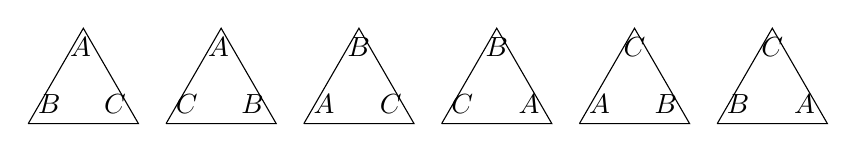
\begin{tikzpicture}[scale=0.7]
        \draw (-1,0)--(1,0)--(0,1.732)--(-1,0);
        \draw (-3.5,0)--(-1.5,0)--(-2.5,1.732)--(-3.5,0);
        \draw (-6,0)--(-4,0)--(-5,1.732)--(-6,0);
        \draw (4,0)--(6,0)--(5,1.732)--(4,0);
        \draw (1.5,0)--(3.5,0)--(2.5,1.732)--(1.5,0);
        \draw (6.5,0)--(8.5,0)--(7.5,1.732)--(6.5,0);
        \node[below] at (-5.05, 1.732) {$A$};
        \node[below] at (-2.55, 1.732) {$A$};
        \node[below] at (-0, 1.732) {$B$};
        \node[below] at (2.5, 1.732) {$B$};
        \node[below] at (5, 1.732) {$C$};
        \node[below] at (7.5, 1.732) {$C$};
        \node[above right] at (-6,0) {$B$};
        \node[above right] at (-3.5,0) {$C$};
        \node[above right] at (-1,0) {$A$};
        \node[above right] at (1.5,0) {$C$};
        \node[above right] at (4,0) {$A$};
        \node[above right] at (6.5,0) {$B$};
        \node[above left] at (-4.05,0) {$C$};
        \node[above left] at (-1.55,0) {$B$};
        \node[above left] at (0.95,0) {$C$};
        \node[above left] at (3.45,0) {$A$};
        \node[above left] at (5.95,0) {$B$};
        \node[above left] at (8.45,0) {$A$};
      \end{tikzpicture}
    \end{center}
  \end{example}

  \begin{example}[Dihedral Group of Order 8]
    The group of rotations and reflections that preserve the structure of a square in $\mathbb{R}^2$. is called the Dihedral Group $\Dih(4)$. 

    \begin{figure}[H]
      \centering 
      \begin{tabular}{|c|c|c|c|c|c|c|c|c|}
        \hline
        & $e$ & $r$ & $r^2$ & $r^3$ & $f$ & $rf$ & $r^2f$ & $r^3f$ \\
        \hline
        $e$ & $e$ & $r$ & $r^2$ & $r^3$ & $f$ & $rf$ & $r^2f$ & $r^3f$ \\
        \hline
        $r$ & $r$ & $r^2$ & $r^3$ & $e$ & $rf$ & $r^2f$ & $r^3f$ & $f$ \\
        \hline
        $r^2$ & $r^2$ & $r^3$ & $e$ & $r$ & $r^2f$ & $r^3f$ & $f$ & $rf$ \\
        \hline
        $r^3$ & $r^3$ & $e$ & $r$ & $r^2$ & $r^3f$ & $f$ & $rf$ & $r^2f$ \\
        \hline
        $f$ & $f$ & $r^3f$ & $r^2f$ & $rf$ & $e$ & $r^3$ & $r^2$ & $r$ \\
        \hline
        $rf$ & $rf$ & $f$ & $r^3f$ & $r^2f$ & $r$ & $e$ & $r^3$ & $r^2$ \\
        \hline
        $r^2f$ & $r^2f$ & $rf$ & $f$ & $r^3f$ & $r^2$ & $r$ & $e$ & $r^3$ \\
        \hline
        $r^3f$ & $r^3f$ & $r^2f$ & $rf$ & $f$ & $r^3$ & $r^2$ & $r$ & $e$ \\
        \hline
      \end{tabular}
      \caption{Multiplication table for $D_4$ using simplified notation.} 
      \label{fig:square_d4_simplified}
    \end{figure}

    Note that this is \textbf{not} the same as the symmetry group of the regular tetrahedron! 
  \end{example} 

  Following this pattern, we can extrapolate to find that the Dihedral group is a symmetry group. 

  \begin{theorem}[Dihedral Groups as Symmetry Groups]
    $\Dih(n)$ is similarly the group of all rotations and reflections that preserve the structure of a regular $n$-gon in $\mathbb{R}^2$. 
  \end{theorem}

  \begin{example}[Groups of Order 3]
    $\Dih(3) \simeq S_{3}$, since permutations of the vertices of a triangle are isomorphic to a permutations of a 3-element set. 
  \end{example}  

  \begin{theorem}[Tip]
    To prove a group homomorphism, show that every element of $G$ and $H$ can be written as a word of certain $g_i$'s in $G$ and then $h_i$'s in $H$, and map the $g_i$'s to $h_i$'s. 
  \end{theorem}

\subsection{Symmetric and Alternating Groups}

  We have seen the natural construction of the symmetric group of a set as the set of bijective transformations. Now the reason that symmetric groups are nice is that we can embed a group into its symmetric group. 

  \begin{theorem}[Cayley's Theorem]
    This applies for both monoids and groups. 
    \begin{enumerate}
      \item Any monoid is isomorphic to a monoid of transformations, i.e. there exists an injective monoid homomorphism 
        \begin{equation}
          f: M \to M^M
        \end{equation}
      \item Any group is isomorphic to a group of transformations, i.e. there exists an injective group homomorphism
        \begin{equation}
          f: G \to \Sym(G)
        \end{equation}
    \end{enumerate}
  \end{theorem}
  \begin{proof}
    Let $(M, \cdot, 1)$ be a monoid. Then we will construct a homomorphism $f: M \to M^M$, the monoid of transformations from $M$ to itself. For any $a \in M$, we define the \textit{left translation} $a_L : x \mapsto ax$. We claim that the set $M^\prime \coloneqq \{a_L \in M^M \mid a \in M \}$ is indeed a monoid. 
    \begin{enumerate}
      \item \textit{Closure}. Given $a, b \in M$, $ab \in M$ and so $ab_L \in M^\prime$. But $(ab_L)(x) = (ab)x = a (bx) = a_L (bx) = a_L (b_L (x)) = (a_L \circ b_L)(x)$, so $ab_L = a_L \circ b_L$. 
      \item \textit{Identity}. $e \in M \implies e_L \in M$ where $e_L : x \mapsto x$. 
    \end{enumerate}
    Next we claim that is is an isomorphism. 
    \begin{enumerate}
      \item This is a homomorphism due to the closure and identity properties proved above. 
      \item It is injective since given $a \neq b$ in $M$, $a_L$ and $b_L$ acts on the identity in different ways $a_L(e) = a \neq b = b_L (e)$, so $a_L \neq b_L$. 
      \item It is surjective by definition. 
    \end{enumerate}
    We have proved for monoids. For groups, we have the additional assumption that inverses exist in $G$, and we must prove that the set of left translations $G^\prime$ is indeed a group. It suffices to prove that inverses exist in $G^\prime$. Given $a \in G$, $a_L \in G^\prime$. But $a^{-1} \in G$ since $G$ is a group, and so $a^{-1}_L \in G^\prime$ as well. We can see that 
    \begin{align}
      (a^{-1}_L a_L) (x) & = (a^{-1} a) x = ex = x \\
      (a_L a^{-1}_L) (x) & = (a a^{-1}) x = ex = x
    \end{align}
    and so indeed $(a^{-1})_L = (a_L)^{-1}$. From this additional fact all the rest follows exactly as for monoids. 
  \end{proof}

  \begin{corollary}[Cayley]
    Every group $G$ is isomorphic to a subgroup of its symmetric group. 
  \end{corollary}

  Now we limit our scope to only finite sets, i.e. finite symmetric groups, which are often called \textbf{permutation} groups. For such finite sets the labeling does not matter since such groups are always isomorphic, so we can say $S = \{1, 2, \ldots, n\}$.

  \begin{theorem}[Symmetric Group as a Symmetry Group]
    The symmetric group $S_n$ is isomorphic to the symmetry group of the $n$-simplex in $\mathbb{R}^{n-1}$. 
  \end{theorem}
  \begin{proof}
    
  \end{proof}

  Now armed with group presentations and generating sets, let attempt to find a group presentation for a permutation group. Given set $S = \{1, 2, \ldots, n\}$, a permutation $\gamma \in \Sym(S)$ is denoted 
  \begin{equation}
    \gamma = \begin{pmatrix} 
      1 & 2 & 3 & 4 & \ldots & n-2 & n-1 & n \\ 
      i_1 & i_2 & i_3 & i_4 & \ldots & i_{n-2} & i_{n-1} & i_n 
    \end{pmatrix} \in \Sym(S)
  \end{equation} 

  We begin by introducing a specific instance of a permutation. 

  \begin{definition}[Cycle Permutation]
    A permutation is said to be \textbf{cyclic} if there exists some subset $A \subset S$ such that $\gamma$ acts as 
    \begin{equation}
      a_1 \mapsto a_2 \mapsto a_3 \ldots \mapsto a_k \mapsto a_1
    \end{equation}
    and leaves the rest unchanged. The notation for this is 
    \begin{equation}
      \begin{pmatrix} a_1 & a_2 & \ldots & a_k \end{pmatrix} \in \Sym(S)
    \end{equation}
    A cycle acting on a subset of 2 elements, i.e. a swap of two elements, is called a \textbf{transposition}. Two cyclic rotations $\gamma_1, \gamma_2$ are \textbf{disjoint} if the subsets that they act on are disjoint: $A \cap B = \emptyset$. 
  \end{definition}

  \begin{example}[Some Cyclic Permutations]
    This notation can be a bit weird, so let's give some simple examples. 
    \begin{enumerate}
      \item $(1 2)$ is a mapping $1 \rightarrow 2,\; 2 \rightarrow 1$. 
      \item $(1 2 3)$ is a mapping $1\rightarrow 2,\; 2 \rightarrow 3,\; 3 \rightarrow 1$. 
      \item $(1 2 3) (4 5)$ is a mapping $1\rightarrow 2,\; 2 \rightarrow 3,\; 3 \rightarrow 1, \;4 \rightarrow 5, \;5 \rightarrow 4$. 
    \end{enumerate}
  \end{example}

  \begin{lemma}
    Every element in finite $S_{n}$ can be decomposed into a partition of cyclic permutations.
  \end{lemma}

  \begin{example}[Cyclic Decomposition of Permutation]
    For the following permutation
    \begin{equation}
      \gamma = \begin{pmatrix} 
        1 & 2 & 3 & 4 & 5 & 6 & 7 & 8 \\ 
        3 & 6 & 5 & 4 & 8 & 2 & 7 & 1 
      \end{pmatrix} = (7)(4)(26)(1358)
    \end{equation} 
  \end{example}

  \begin{theorem}[Transpositions]
    The set of all transpositions forms a generating set of $S_{n}$. 
  \end{theorem}

  Recognizing that the set of transpositions is the generating set of the permutation group. In fact, transpositions allow us talk about the parity of an arbitrary permutation, through its signature. 

  \begin{definition}[Signature]
    The \textbf{signature} of a permutation is a homomorphism
    \begin{equation}
      \sign : S_{n} \longrightarrow \{1, -1\}
    \end{equation}
  \end{definition}

  \begin{lemma}
    The signature of a permutation changes for every transposition that is applied to it. 
  \end{lemma} 

  Now we are ready to introduce another fundamental type of group. 

  \begin{definition}[Alternating Group]
    The \textbf{alternating group} is the kernel of the signature homomorphism $\sign: S_n \to \{\pm 1\}$. 
    \begin{equation}
      A_n \coloneqq \ker{\sign}
    \end{equation}
    It is the set of even permutations with order $n!/2$.\footnote{Note that the set of odd permutations do not form a group, since the composition of two odd permutations (each having signature $-1$ is an even permutation. }
  \end{definition}

  This construction might seem arbitrarily specific to study so early into algebra, but as we will see later, we will find that that for $n \geq 5$, they will be simple groups that can't be decomposed and therefore fundamental in a sense. 

  \begin{example}[Low Order Symmetric Groups]
    \begin{enumerate}
      \item $S_{0}$ is the set of all permutations on the \textbf{null set}. $S_{1}$ is the set of all permutations on the \textbf{singleton set}. Both sets have cardinality 1 and the element is \textbf{trivial}. Note that $S_{1} = A_{1}$. 
      \item $S_{2}$ is a cyclic, abelian group of order 2 consisting of the identity permutation and the transposition of two elements. 
      \item $S_{3}$ is the first cyclic, nonabelian group, with order 6. $S \simeq \Dih(3)$, which can be seen as the group of rotations and reflections on the equilateral triangle, and the elements of $S_{3}$ equate to permuting the vertices on the triangle. 
    \end{enumerate}
  \end{example}

  In lecture, we talked about the number of all finite set is $e$. Since $n!$ is the order of permutation groups, i.e. the order of automorphism groups, we can sum their inverses over all $n \in \mathbb{N}$ to get $e$.  

\subsection{Group Actions} 

  We have studied the general properties of groups, but historically group theory arose from the study of transformation groups (which is why I also introduced is so early on). These transformation groups can be thought of as an abstract group it itself, but another way to interpret it is to see how it \textit{acts} on a set. 

  \begin{definition}[Group Action]
    Let $G$ be a group, $S$ a set. Then, a (left) group action of $G$ on $S$ is a function
    \begin{equation}
      \sigma: G \times S \to S, \qquad \sigma(g, a) = g \cdot a 
    \end{equation}
    satisfying two axioms. 
    \begin{enumerate}
      \item \textit{Identity}. $\forall a \in S, \sigma(e, a) = a$. 
      \item \textit{Compatibility}. $\forall g, h \in G \text{ and } \forall x \in X, \sigma(gh, x) = \sigma(g, \sigma(h, x))$.
    \end{enumerate}
    The group $G$ is said to \textbf{act on} $S$, and the evaluation $\sigma(g, a)$ can be interpreted as the result after transforming $a$ through $g$. 
  \end{definition}
  
  \begin{theorem}[Group Action as a Homomorphism onto the Symmetric Group]
    We have the immediate facts. 
    \begin{enumerate}
      \item For a fixed $g \in G$, the group action $\sigma_g (s) \coloneqq \sigma(g, s): S \to S$ is a bijection, i.e. an element of $\Sym(S)$. The inverse is the function mapping $x \mapsto \sigma(g^{-1}, x)$.
      \item The map from $G$ to $\Sym(S)$ defined by $g \mapsto \sigma_g$ is a homomorphism. 
    \end{enumerate}
  \end{theorem}
  \begin{proof}
    
  \end{proof}

  \begin{example}[Permutations and Dihedral Groups as Group Actions]
    In fact, we have seen two concrete examples of such group actions. 
    \begin{enumerate}
      \item The permutation group acts on the set $S = \{1, \ldots, n\}$ by permuting its elements. It also acts on a set of $n$-simplexes by rotating/flipping them. 
      \item The dihedral group acts on the set of regular $n$-gons by rotating/flipping them. 
    \end{enumerate}
  \end{example}


